\scanpage{12}
\deleted{\unsure{fixe, mettons} $\mathbf C$ \unsure{ici}) sont déterminés à \unsure{cat.} alg. près. \unsure{N. m.} Nous \unsure{examinons} la

\uline{Conjecture}\inserted{\uline{transcendance}} Si $k$ est \unsure{quasi-modulaire|quasi-minimal} pour $M$, alors
\[
\operatorname{deg\,tr}(k(g_0))=\dim G^{\unsure{u}}\quad(=\dim G-1),
\]
i.e. $\unsure{\xi_0|g_0}$ \inserted{(localisé en $g_0$)} est un point \uline{maximal} de $G^{\unsure{u}}$ (du moins si $G$ donc $G^{\unsure{u}}$ connexe).}

\margin{\unsure{calcul} pour courbes elliptiques à invariant transcendant et $\tau$ algébrique.....}

\deleted{\uline{Corollaire.} \inserted{\figure{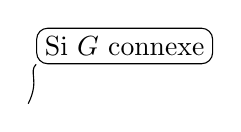
\begin{tikzpicture}[baseline=(n.base)]\node[draw,rounded corners=4pt,inner sep=3pt] (n) {Si $G$ connexe};\draw (n.south west) .. controls +(-.1,-.1) and +(.15,.3) .. ++(-.1,-.5);\end{tikzpicture}}} $G^{\unsure{u}}$ est le groupe algébrique engendré par $g_0$. Donc $G$ est le groupe algébrique engendré par $g_0$ et $j(G_m)$ (les homothéties). Enfin $G$ est engendré sur $k$ par $g$ si $G^{\unsure{u}}$ est $\frac12$ simple et $\pi$ \unsure{non|un} \unsure{algébrique} sur $k$ \deleted{\illegible{1}} ...}

\margin{et en général \deleted{\unsure{$G^u$}\quad\unsure{R un alg.}\quad\unsure{sur $k$ ?}}}

\deleted{Contient le th. de Schneider, pour les courbes elliptiques sans mult. complexe. En fait, il signifie que le degré de transc. du système
\[
\begin{array}{cccc}
(\unsure{\zeta|\xi}^{-1}\omega_1,&\unsure{\zeta|\xi}^{-1}\omega_2,&\unsure{\zeta|\xi}^{-1}\eta_1,&\unsure{\zeta|\xi}^{-1}\eta_2)\\
\text{''}&\text{''}&\text{''}&\text{''}\\
\omega'_1&\omega'_2&\eta'_1&\eta'_2
\end{array}
\]
sur $\mathbf Q$ est $3$ \deleted{\unsure{est}} (la seule relation étant $\omega'_1\eta'_2-\omega'_2\eta'_1=1$, \unsure{c.o.} l'équation de $G^{\unsure{u}}=\mathrm{SL}(2)\subset G=\mathrm{GL}(2)$) pour une courbe elliptique sans mult. complexe définie sur un corps de nbs alg. (disons sur $\overline{\mathbf Q}$).

Si l'invariant $j$ est transcendant, on \unsure{trouvera} que $(j,\omega'_1,\omega'_2,\eta'_1,\eta'_2)$ ont le degré de \uline{trans. $4$} sur $\mathbf Q$.}
\margin{11}
